\label{sec:IF_SBND}
The SBND experiment is designed to build upon the many years of LArTPC R$\&$D and serve as a test-bed for the future long baseline neutrino experiment. SBND's design is to construct a membrane cryostat in a new experiment hall located 110 meters from the BNB target. The cryostat will house the full TPC consisting of one central cathode plane assembly (CPA) and four anode plane assemblies (APAs) which will have three wire planes with three millimetre spacing (similar to the ICARUS design) and the first two induction planes oriented at $\pm 30^{\circ}$ to the beam axis and the final plane oriented vertically. SBND will be a 5.0~m~$\times$~4.0~m~$\times$~4.0~m (l$\times$w$\times$h) TPC with 112 tons of active volume. SBND will also have a light detection system based on a hybrid of the ICARUS cryogenic PMT's and the proposed DUNE light-guide with silicon photomultiplier (SiPMs) on the end. This light detection system will be embedded behind the APA structure on both sides of the TPC. 

%\begin{figure}[htb]
%\centering
%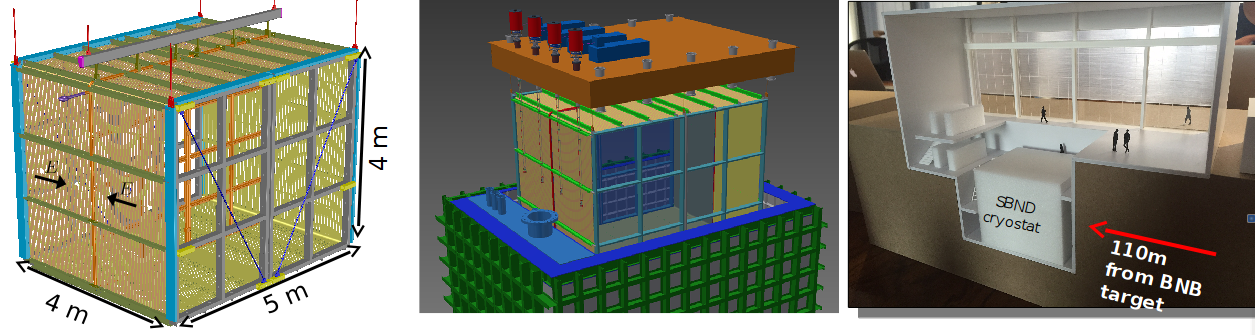
\includegraphics[width=0.75\textwidth]{images/sbnd.png}
%\caption[]{Conceptual design of the SBND TPC, cryostat, and detector hall.}
%\label{fig:sbnd}
%\end{figure}

One new unique aspect of the SBND detector will be the inclusion of the entire front end readout chain being moved into the liquid argon. The front end electronics are composed of 16-channel analogue front end ASIC which provides amplification and shaping, a 16 channel analogue to digital converter ASIC which provides digitization, buffering, and multiplexing as well as a cold FPGA which provides second multiplexing and voltage regulation. This technical improvement in readout electronics will provide improved signal-to-noise as well as allow for the development of an efficient zero-suppression scheme implemented in the FPGA to greatly reduce the total data volume. Many bench tests of the readout electronics have been performed and show excellent performance. The full integration test with an operating TPC, however, has not been successfully performed (given the many problems seen by the DUNE 35ton prototype) and is an absolutely necessary service task the UTA group is planning to spearhead. 

%%%%%%%%%%%%%%%%%%%%%%%%%%%%%%%%%%%%%%%%%%%%%%%%%%%%%%%%%%%%%%%%%%%%%
\subsection{SBND Cold Electronics Teststand}\label{sec:SBNDTeststand}
%%%%%%%%%%%%%%%%%%%%%%%%%%%%%%%%%%%%%%%%%%%%%%%%%%%%%%%%%%%%%%%%%%%%%
Figure \ref{fig:teststand} shows a schematic of what a test-stand would look like utilizing the ``Blanche'' cryostat currently installed at the Proton Assembly Building (PAB)at Fermilab. This cryostat is engineered to have a delivery system for purified liquid argon in addition to a system to circulate, re-condense, and purify boil-off argon. An identical cryostat is currently being built and will be delivered to UTA late 2016. This cryostat will work in conjunction with the liquid argon purification system currently in operation at UTA. This system is built using start-up funds from P.I. Asaadi and will allow UTA to play an important role in detector R$\&$D in the coming years. 

\begin{figure}[htb]
\centering
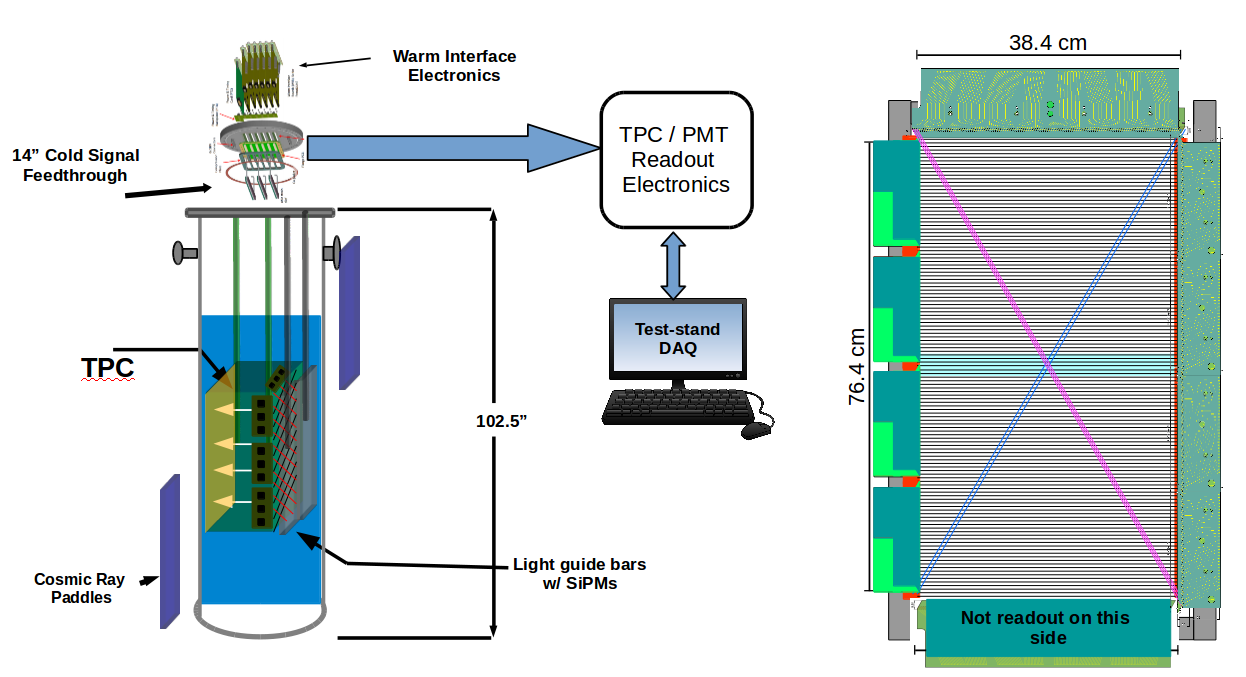
\includegraphics[width=0.68\textwidth]{images/teststand3.png}
\caption[]{Conceptual design of the SBND cold electronics vertical slice test-stand. Integration of both cold or warm electronics, light collection system, cosmic ray paddles and warm interface electronics allows for a complete testing of the entire readout system prior to deployment in the experiment and to provide a platform for DAQ debugging outside the actual the experiment. The current design has 768 channels (256 collection, 512 induction) utilizing six motherboards for SBND.}
\label{fig:teststand}
\end{figure} 

Inside the cryostat, a small scale TPC equipped with prototype SBND cold readout electronics installed along side a pair of light guide bars can be deployed and read out through a 14'' inch cold signal feedthrough as designed for the SBND detector. External to the cryostat, scintillator paddles can be positioned to act as an external trigger. Since the cryostat is a copy of an existing one at FNAL, upon the completion of the test the top flange and the TPC detector will be shipped to FNAL for longer term use for SBND (and potentially other future LArTPCs). Additional material costs, such as the electronics, power supplies and cabling are expected to be provided by SBND project funds and Asaadi's start-up funds.

The test-stand enables a robust set of tests for the integration of many newly developed readout electronic components prior to their deployment in the experiment, providing ample opportunities to discover and fix any unforseen problems, such bias voltage line for the TPC wires causing pick-up noise or cross-talk between the light detection system and the TPC readout.   In addition, DAQ software can also be tested using the test stand since it can be equipped with a complete chain of the DAQ system.  Such software development can be expanded to development and testing of common DAQ and other software packages for LArTPC, such as artDAQ and LArSoft. 

%This critical step was not taken during the MicroBooNE assembly and as a result a number of problems with the readout electronics were not detected in advance of attempting to commission the detector. These problems included the bias voltage line for the TPC wires behaving in an unexpected way and causing pick-up noise to be seen on the electronics, cross-talk between the light detection system and the TPC readout, and the incorrect configuration of electronics settings because of software bugs. While many of these issues were able to be solved during the commissioning phase, they slowed the progress of transitioning to data taking and caused unnecessary harm to the experiment. Moreover, this test-stand will provide a platform for testing and debugging of the DAQ software and readout electronics configuration without interrupting the operation of the SBND experiment. 

%The postdoctoral researcher and graduate student will be developing the readout software into a common DAQ software package used by other LArTPC based experiments known as the artDAQ framework. This common platform ensures that the work done by those supported in this proposal can have a greater impact on future planned LArTPCs as well as allowing them to benefit from the work that has already been done by others.

%Finally, such a test-stand can provide an R$\&$D platform for long term testing of future readout components as well as software development for online triggers and zero-suppression schemes without risking downtime on operating neutrino detectors. The trigger schemes envisioned include utilizing multi-core graphical processing units to do online TPC based triggering for rare search events such as proton decay and supernova neutrino triggering. Moreover, by providing a platform for the development of LArTPC's DAQ systems into a common platform such as artDAQ, a greater push to the integration of the data, simulation, and analysis into one common software platform can be accomplished. The events processed utilizing the artDAQ software are immediately readable by the common liquid argon software framework known as LArSoft. Thus, working on this system and the associated neutrino detectors DAQ help promote the use of a common software framework.


%%%%%%%%%%%%%%%%%%%%%%%%%%%%%%%%%%%%%%%%%%%%%%%%%%%%%%%%%%%%%%%%%%%%%
\subsection{SBND Construction, Installation, and Commissioning}\label{sec:SBNDBulid}
%%%%%%%%%%%%%%%%%%%%%%%%%%%%%%%%%%%%%%%%%%%%%%%%%%%%%%%%%%%%%%%%%%%%%
The UT Arlington group is positioned to play a major role in the construction, installation and commissioning of the SBND detector and its DAQ system. Given Asaadi's experience on MicroBooNE and LArIAT in which he played a lead role of TPC expert during construction, commissioning, and operations as well as the experience of the post-doctoral researchers already with the group (Falcone on ICARUS and Chatterjee on LArIAT) UTA can offer hands-on leadership during the construction phase of the experiment.

During the construction phase for the TPC (foreseen in mid 2017 through mid 2018), Falcone is expected to be in residence at FNAL and will be spending 50$\%$ of his time on SBND. During that same time, a to-be-named post-doc will join him at FNAL with a focus on SBND TPC construction. Having these two present will allow for a rapid ramp-up on the project. At the same time, the cold electronics test-stand is expect to be moved from UTA to FNAL for operations. A graduate student, Zach Williams is expected be on SBND and be in residence at FNAL in the summer 2017.  With his time already spent on UTA cold electronics test stand, continuing to contribute to the DAQ development and aiding in the construction and installation of the cold electronics on the TPC will enable him to make significant contributions to the experiment.  Asaadi and Yu plan to spend a significant portion of their time at FNAL in the bottom half of 2017 and top half of 2018, respectively, to help oversee these activities and contribute to the construction of the experiment.

Following the construction and installation phase, one post-doc and one graduate student are expected to stay with the SBND experiment, spending a significant portion of their time and play a role as detector experts during the commissioning and initial data taking. The aim here is to share their expertise across the SBN program, but to have a reliable source of experts in residence at FNAL for SBND.  While stationed at UTA, graduate and undergraduate students will have the opportunity to take remote shifts on this experiment utilizing UTA's remote shift station currently residing in UTA's cryogenics lab. This remote station has already been used to take shifts on the LArIAT experiment and is currently being commissioned to be able to take remote shifts for the MicroBooNE experiment. UTA group plans on expanding this station to play a role as a sattellite control station for LArTPC experiments, namely MicroBooNE, SBND, ICARUS and DUNE, coming online well in advance of SBND data taking.  

%%%%%%%%%%%%%%%%%%%%%%%%%%%%%%%%%%%%%%%%%%%%%%%%%%%%%%%%%%%%%%%%%%%%%
\subsection{SBND Data Analysis}\label{sec:SBNDDataAnalysis}
%%%%%%%%%%%%%%%%%%%%%%%%%%%%%%%%%%%%%%%%%%%%%%%%%%%%%%%%%%%%%%%%%%%%%
SBND will provide important physics measurements during its early operations in addition to providing an overall flux normalization to the key SBN oscillation analysis. Critically, SBND will collect very quickly statistics to confirm the nature of the MiniBooNE excess as measured by MicroBooNE. If MicroBooNE were to confirm the MiniBooNE excess as originating from electron-like sources, SBND could quickly measure if there is an oscillation component to the electron-like signal by measuring the rate as seen in the near detector. Conversely, if MicroBooNE were to determine the MiniBooNE excess as originating from photon-like sources, SBND can cross-check if the source is an unaccounted for beam like background or coming from cosmogenic like backgrounds. Regardless of the outcome, SBND will play a critical role in quickly collecting high statistics data as the near detector to the SBN program.

SBND will also provide critical neutrino cross-section measurements at a statistical precision unprecedented by any other LArTPC. SBND will collect approximately two million neutrino interactions per 2.2$\times 10^{20}$ protons  on target (roughly one year of running). With 1.5 million $\nu_{\mu}$ charged current interactions and 12,000 $\nu_{e}$ charged current interactions in one year. With such statistics, many precision cross-section measurements (e.g. double differential) become possible and improvements on first and second generation analyses from MicroBooNE can be explored in the first year of data taking.

\begin{figure}[htb]
\centering
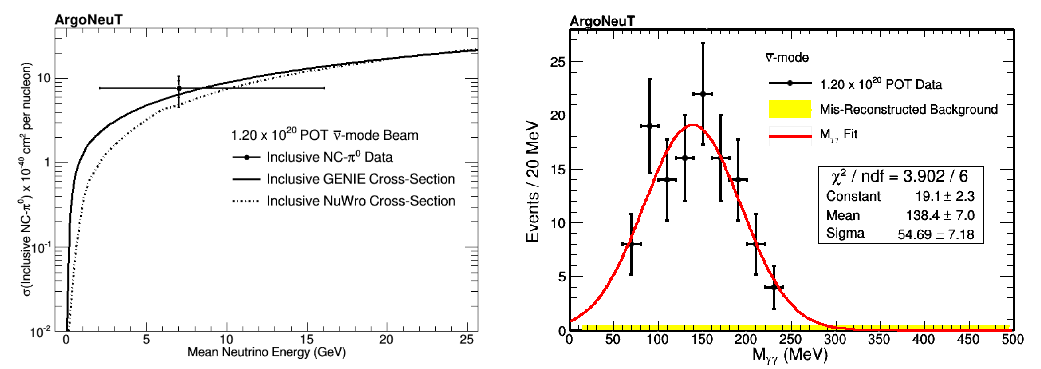
\includegraphics[width=0.95\textwidth]{images/ArgoNeuTPizeroResult.png}
\caption[]{The only existing NC-$\pi^0$ measurement on argon from the ArgoNeuT collaboration. P.I. Asaadi was the leading analyzer on this result and intends to leverage the large statistics sample to be collected by SBND to provide a low energy measurement of this cross-section, which is one of the leading systematics in the both the short and long-baseline oscillation results.}
\label{fig:argoneutpizero}
\end{figure} 



Furthermore, by collecting approximately 100,000 NC$\pi^{0}$ events per year a full characterization of the leading background cross-section to the long baseline CP-violation analysis can be performed. Figure \ref{fig:argoneutpizero} shows the only neutral current $\pi^0$ result on an argon nucleus from the ArgoNeuT collaboration \cite{}. This result was lead by P.I. Asaadi and thus positions the UTA group to uniquely lead this next generation analysis with a much larger statistics sample. The elimination of this systematic uncertainty in the cross-section will improve the experimental reach of the future planned DUNE experiment as well as benifit the short-baseline $\nu_{e}$ oscillation analysis.
